\documentclass[12pt, twoside]{article}
\usepackage{jmlda}
\bibliographystyle{jmlda-rus.bst}
\newcommand{\hdir}{.}

\usepackage{graphicx}
%\graphicspath{ {../fig/} {.}}
%\usepackage[ruled,vlined]{algorithm2e}


\begin{document}

\title
    [Дифференцируемый алгоритм поиска архитектуры модели с контролем её сложности] % краткое название; не нужно, если полное название влезает в~колонтитул
    {Дифференцируемый алгоритм поиска архитектуры модели с контролем её сложности}
\author
    [К.\,Д.~Яковлев, О.\,С.~Гребенькова, О.\,Ю.~Бахтеев] % список авторов (не более трех) для колонтитула; не нужен, если основной список влезает в колонтитул
    {К.\,Д.~Яковлев, О.\,С.~Гребенькова, О.\,Ю.~Бахтеев} % основной список авторов, выводимый в оглавление
    [К.\,Д.~Яковлев, О.\,С.~Гребенькова, О.\,Ю.~Бахтеев] % список авторов, выводимый в заголовок; не нужен, если он не отличается от основного
\email
    { iakovlev.kd@phystech.edu; grebenkova.os@phystech.edu; bakhteev@phystech.edu}

\abstract
    {В работе исследуется задача построения модели глубокого обучения. Предлагается метод поиска архитектуры модели, позволяющий контролировать её сложность с небольшими вычислительными затратами. Под сложностью модели понимается минимальная длина описания,
минимальное количество информации, которое требуется для передачи информации о модели и выборке. В основе метода лежит дифференцируемый алгоритм поиска архитектуры модели (DARTS). Предлагается использовать гиперсеть в качестве функции релаксации.  Под гиперсетью понимается модель, генерирующуя параметры другой модели. Предложенный метод позволяет контролировать сложность модели в процессе поиска архитектуры. Для оценки качества предлагаемого алгоритма проводятся эксперименты на выборках MNIST и CIFAR-10.
	
\bigskip
\noindent
\textbf{Ключевые слова}: \emph {дифференцируемый алгоритм поиска архитектуры; глубокое обучение; гиперсети; нейронные сети; контроль сложности модели}
}



%данные поля заполняются редакцией журнала
%\doi{10.21469/22233792}
\receivedRus{25.02.2021}
\receivedEng{February 25, 2021}


\maketitle
\linenumbers

\section{Введение}

В последнее время растет интерес к разработке алгоритмических решений для автоматизации процесса проектирования архитектуры. Лучшие существующие алгоритмы поиска архитектуры требуют больших вычислительных затрат, несмотря на их высокое качество.

В данной работе рассматривается задача поиска архитектуры модели глубокого обучения с контролем её сложности. В качестве базового алгоритма используется дифференцируемый алгоритм поиска архитектуры (DARTS) \cite{journals/corr/abs-1806-09055}. Данный метод решает задачу поиска архитектуры модели путем перевода пространства поиска из дискретного в непрерывное представление. В связи с этим появляется возможность использовать градиентные методы оптимизации, позволяющие использовать меньше вычислительных ресурсов, чем методы, работающие на дискретном множестве. Данный алгоритм универсален для работы как со сверточными, так и с рекуррентными нейронными сетями.

В работе \cite{journals/corr/abs-2002-05283} стабильность алгоритма DARTS была поставлена под сомнение. Одним из источников нестабильности является этап получения фактической дискретной архитектуры из архитектуры непрерывной смеси. На этом этапе часто наблюдается снижение качества модели. Это связано с тем, что алгоритм сходится в узкий регион, поэтому  небольшие возмущения архитектуры ведут к значительному понижению качества на валидационной выборке. 

В работе \cite{journals/corr/abs-1911-12126} было замечено, что операция $softmax$ обладает существенным недостатком. Оказывается, что пропуск соединений постепенно становится доминирующим в процессе оптимизации. Вес данного соединения увеличивается гораздо быстрее, чем у его конкурентов. В связи с этим предлагается использовать сигмоидную  функцию потерь. Таким образом, каждая операция может давать существенный вклад независимо от других. В нашей работе предлагается в качестве функции релаксации использовать гиперсеть \cite{journals/corr/HaDL16}. Подход заключается в использовании небольшой сети для генерации весов операций.
 Предлагаются альтернативные подходы к решению задачи поиска архитектуры модели. В работе \cite{journals/corr/abs-2006-10355} формулируется задача обучения распределению. Веса смешанной операции подчинены распределению Дирихле, так как они определены на вероятностном симплексе. Таким образом, задача поиска архитектуры сводится к поиску параметров распределения Дирихле.

В работе \cite{journals/corr/abs-1912-12814} строится алгоритм поиска нейронной архитектуры с ограниченным ресурсом (RC-DARTS). К базовому алгоритму DARTS добавляются ресурсные ограничения, такие как размер модели и вычислительная сложность. Для решения задачи условной оптимизации вводится алгоритм итерационной проекции, поскольку функции ограничений невыпуклые. В нашей работе для контроля сложности используется гиперсеть.


Вычислительный эксперимент проводится на выборках MNIST\cite{lecun-mnisthandwrittendigit-2010} и CIFAR-10\cite{cif}.

\section{Постановка задачи}

\subsection{Дифференцируемый алгоритм поиска архитектуры}

Поставим задачу поиска архитектуры ячейки.
 Пусть внутри ячейки есть $N$ занумерованных узлов, пердставленных в виде ориентированного ациклического графа. Каждому ребру $(i, j)$ поставлена в соответствие операция $o^{(i, j)} \in \mathcal{O}$, где $\mathcal{O}$ -- множество операций. Значения в каждом из промежуточных узлов $x^{(j)}$ определяются через значения в узлах с меньшим номером:
 
 \begin{equation}
 x^{(j)} = \sum_{i < j}o^{(i, j)}(x^{(i)})
 \end{equation}
 
 Таким образом, задача поиска архитектуры сводится к задаче выбора операций между узлами ячейки. Для того, чтобы свести задачу дискретной оптимизации к задаче непрерывной оптимизации, введем смешанную операцию для каждого ребра $(i, j)$:

\begin{equation}
\hat{o}^{(i, j)}(x) = \sum_{o\in \mathcal{O}} \frac{\exp(\alpha_o^{(i, j)})}{\sum_{o'\in\mathcal{O}} \exp(\alpha_{o'}^{(i, j)})}o(x),
\end{equation}
где $\alpha_o^{(i, j)}$ обозначает соответствующий вес операции $o$ на ребре $(i, j)$. Таким образом, каждому ребру $(i, j)$ ставится в соответствие вертор $\alpha^{(i, j)}$ размерности $|\mathcal{O}|$. Пусть $\alpha = [\alpha^{(i, j)}]$. Сформулируем двухуровневую задачу оптимизации:

\begin{equation}
\begin{aligned}
\min_{\alpha}\mathcal{L}_{val}(\mathbf{w}^*(\alpha), \alpha),\\
 \mathrm{s.t.}\quad \mathbf{w}^* = \arg\min_{\mathbf{w}}\mathcal{L}_{train}(\mathbf{w}, \alpha)
 \end{aligned}
\end{equation}
Здесь $\mathcal{L}_{val}$ и $\mathcal{L}_{train}$ функции потерь модели на валидации и на обучении соответственно.


\begin{algorithm}[H]
\begin{algorithmic}[1]
\caption{DARTS -- Differentiable Architecture Search}
\label{alg:darts}
\STATE Для каждого узла создадим смешанную операцию $\hat{o}^{(i, j)}$, параметризованную $\alpha^{(i, j)}$
\WHILE{алгоритм не сошелся} 
\STATE  обновим $\alpha$, сделав градиентный шаг вдоль $\nabla_\alpha \mathcal{L}_{val}(\mathbf{w} - \xi\nabla_{\mathbf{w}}\mathcal{L}_{train}(\mathbf{w}, \alpha), \alpha)$
\STATE обновим веса $\mathbf{w}$, делая градиентный шаг вдоль $\nabla_\mathbf{w}\mathcal{L}_{train}(\mathbf{w}, \alpha)$
\ENDWHILE
\STATE получить окончательную архитектуру из полученного в результате алгоритма $\alpha$
\end{algorithmic}
\end{algorithm}

Дискретная архитектура получается следующим образом:

$$o^{(i, j)} =\arg\max_{o\in\mathcal{O}}\alpha_o^{(i, j)}$$

\subsection{Линейная гиперсеть}

Пусть $\Lambda$ --  множество параметров, контролирующие сложность модели. Под гиперсетью мы будем понимать следующее отображение:

\begin{equation}
	\mathbf{G} : \Lambda \times \mathbb{U} \rightarrow \mathbb{A},
\end{equation}
где $\mathbb{A}$ -- пространство весов операций $\alpha^{(i, j)}_o$, а $\mathbb{U}$ -- множество параметров гиперсети.
В данной работе для получения весов операций используется линейная гиперсеть:
 
 \begin{equation}\label{hypernet}
 \mathbf{G}_{\text{linear}}(\lambda) = \lambda \mathbf{b}_1 + \mathbf{b}_2,
 \end{equation}
 где $\mathbf{b}_1, \mathbf{b}_2$ -- обучаемые параметры гиперсети.
 
 \subsection{Алгоритм DARTS с контролем сложности}
 
 В качестве базового алгоритма используется алгоритм \ref{alg:darts}. Одним из основных отличий является то, что смешанная операция записывается следующим образом:
 
 $$\hat{o}^{(i, j)} = \sum_{o\in \mathcal{O}}\alpha^{(i, j)}_oo(x)$$
 Кроме того, сложность модели определяется параметром $\lambda$ гиперсети. Остальные шаги алгоритма остаются без изменений.
 
 \section{Вычислительный эксперимент}
 
 \subsection{Базовый эксперимент}
 Целью базового эксперимента является получение зависимости качества работы алгоритма DARTS с регуляризатором от количества эпох при разных значениях параметра регуляризации.
 
 Предлагается использовать алгоритм DARTS с регуляризатором $\lambda_{\text{reg}}\sum_{i=1}^{\dim\alpha}\mathbf{v}_i|\alpha_i|$ в качестве второго слагаемого в функции потерь, где $\mathbf{v}$ -- веса типов операции. Вычислительный эксперимент проводится на выборке MNIST\cite{lecun-mnisthandwrittendigit-2010}, которая представляет собой набор рукописных цифр.
 
Эксперимент запускался 5 раз при значениях $\lambda_{\text{reg}} \in \{0.1, 1, 10, 100\}$. На рисунке \ref{fig:basic_exp} представлен график зависимости точности (precision) модели от числа эпох.

График показывает, что при большом значении параметра регуляризации качество сильно падает. Это связано с тем, что в этом случае не выгодно брать операции с большим весом. Таким образом, модель становится переупрощенной.

 Также из графика видно, что при $\lambda \in \{0.1, 10\}$ качество модели значительно возрастает, что связано с тем, что в архитектуре появляются операции, имеющие высокий вес в регуляризаторе.

\begin{figure}[H]
\centering
  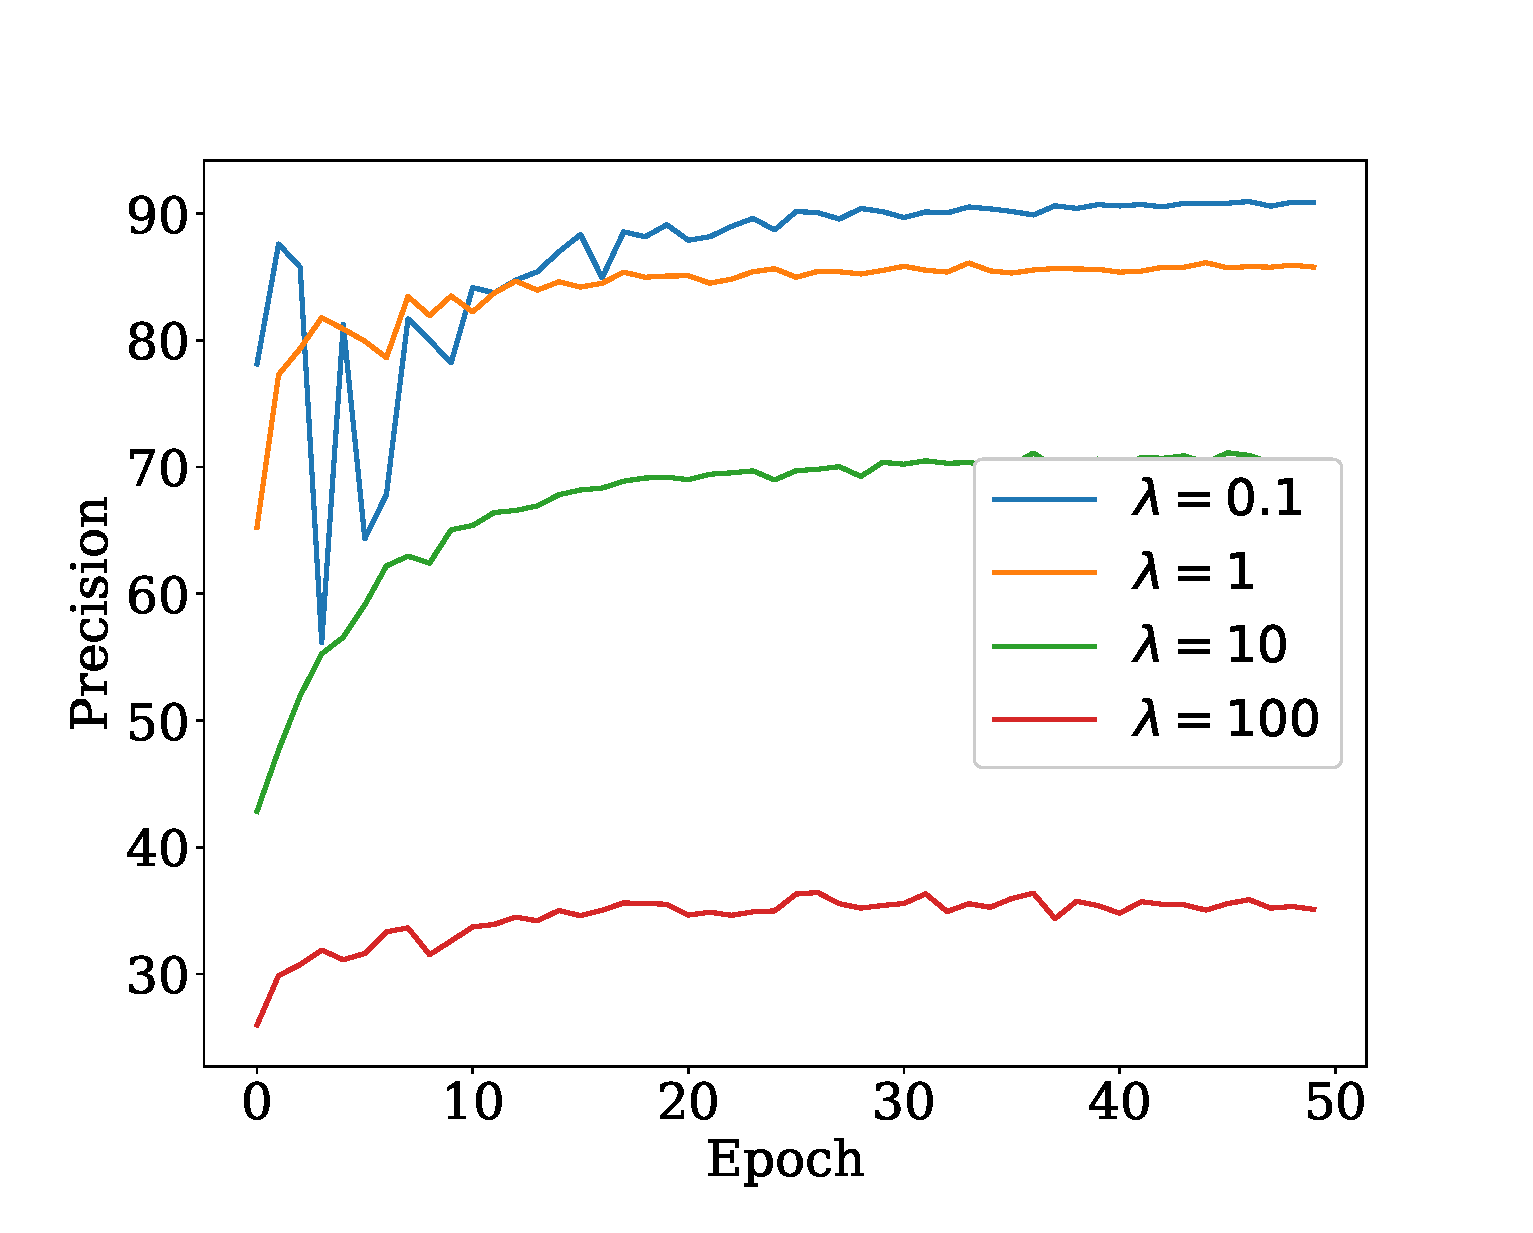
\includegraphics[width=0.8\textwidth]{basic_exp.eps}
  \caption{Зависимость точности модели от числа прошедших эпох для разынх параметров регуляризации}
  \label{fig:basic_exp}
\end{figure}

\subsection{Основной эксперимент}

Целью основного эксперимента является получение зависимости качества работы предложенного метода от параметра гиперсети $\lambda \in \{0.1, 1, 10, 100\}$. Эксперимент проводится на выборке MNIST \cite{lecun-mnisthandwrittendigit-2010}. Рассматривался поиск архитектуры сверночной нейронной сети с одним слоем и четырьмя узлами. Контроль сложности производился линейной гиперсетью \ref{hypernet}. Обучение проводилось на протяжении 100 эпох. Эксперимент запускался 5 раз. 

\begin{figure}[H]
\centering
  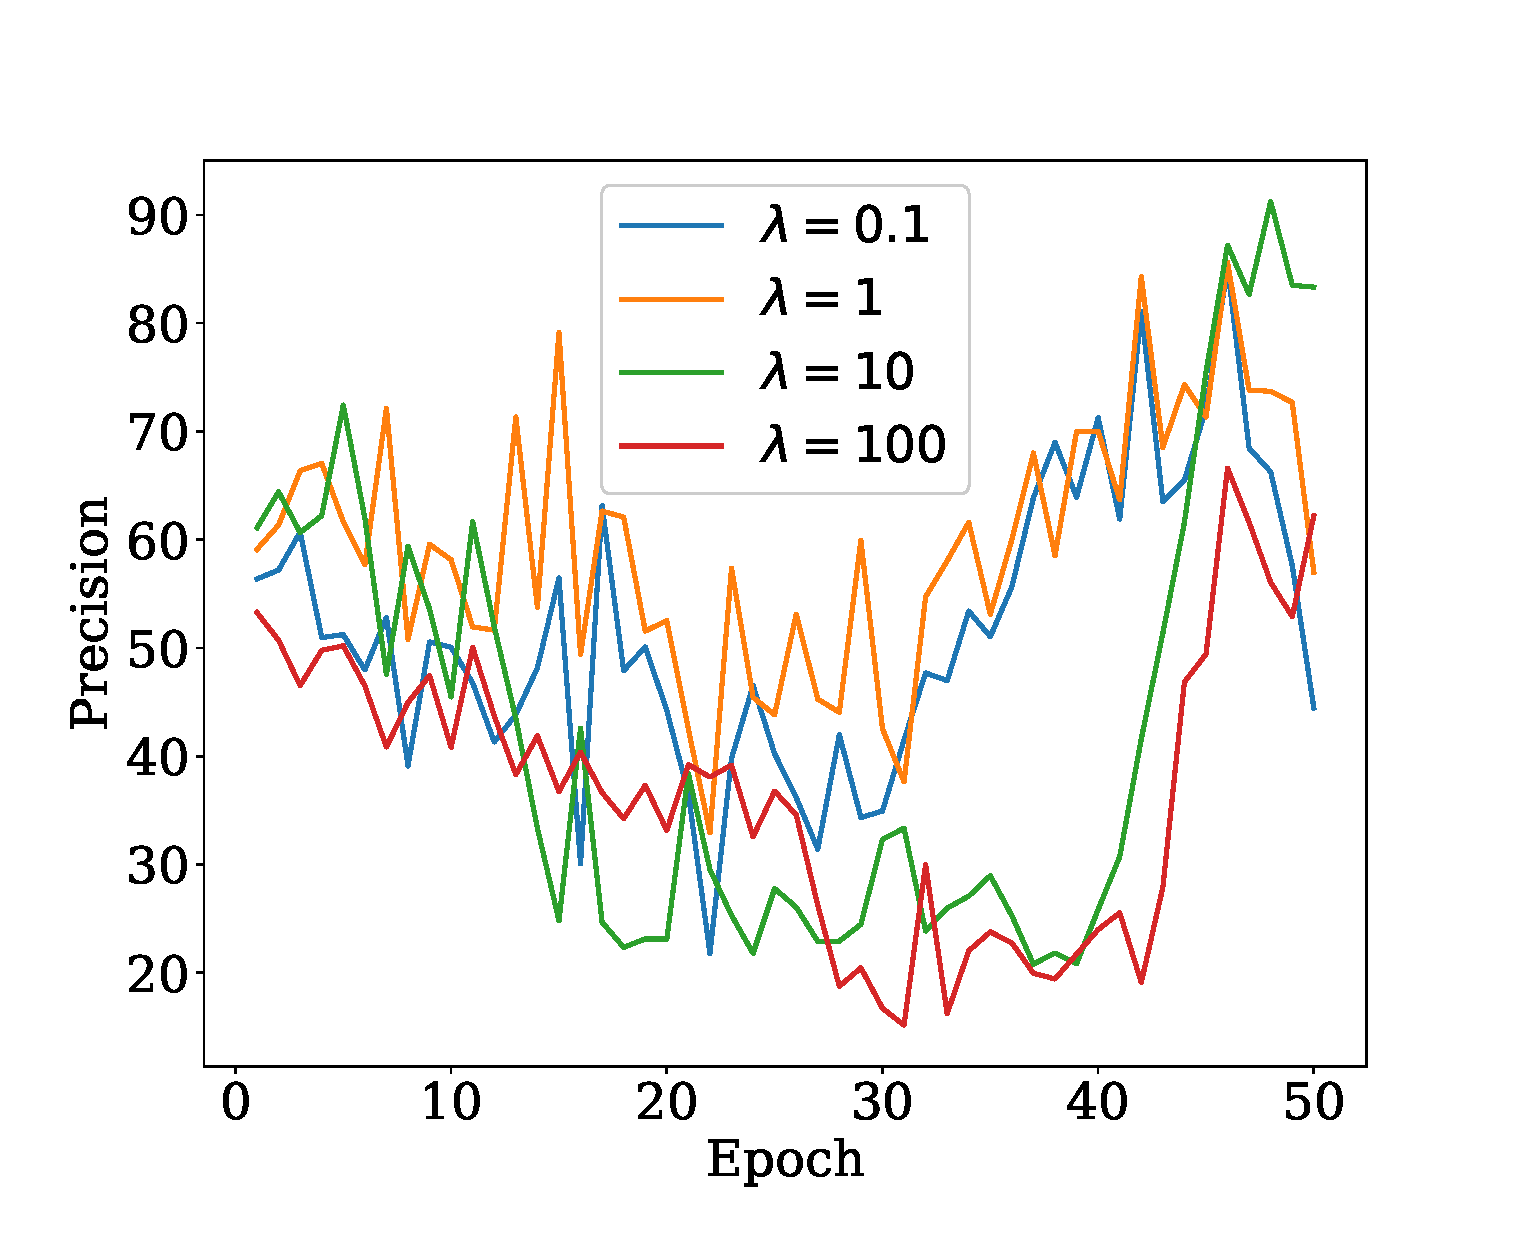
\includegraphics[width=0.8\textwidth]{main_exp.eps}
  \caption{Зависимость усредненной по 5 запускам точности модели от числа прошедших эпох для разных параметров $\lambda$ гиперсети.}
  \label{fig:main_exp}
\end{figure}

На рисунке \ref{fig:main_exp} представлена зависимость усредненной точности (precision) от числа прошедших эпох. Из графика видно, что модели недообучены. Точность начинает значительно возрастать только после 35 эпохи. Для того, чтобы делать дальнейшие выводы, необходимо запустить эксперимент на большем количестве эпох.
 

%%%% если имеется doi цитируемого источника, необходимо его указать, см. пример в \bibitem{article}
%%%% DOI публикации, зарегистрированной в системе Crossref, можно получить по адресу http://www.crossref.org/guestquery/
\newpage
\bibliography{Version1.bib}
\end{document}

